\hypertarget{materialen-en-software}{%
\section{Materialen en software}\label{materialen-en-software}}

Een hand is anatomisch gezien een complex ledemaat. Een nabootsing van
een hand kost dan ook onwijs veel tijd, energie en materialen om te
maken. Bij het maken van een prothese moet er veel rekening worden
gehouden met de materiaalkeuze. Wij zullen de opties voor de materialen
aan de binnen- en buitenkant van de hand en de opties voor software
toelichten.

\hypertarget{materialen-aan-de-buitenkant-van-de-hand}{%
\subsection{Materialen aan de buitenkant van de
hand}\label{materialen-aan-de-buitenkant-van-de-hand}}

Bij het kiezen van een printmateriaal, zijn er een paar overwegingen die
er moeten worden gemaakt. Je wilt dat het materiaal sterk is. Het moet
sterk genoeg zijn om niet zomaar kapot te gaan maar tegelijkertijd zacht
genoeg dat je het nog wel bewerkbaar is. Ook moet het 3D printbaar zijn.
Dit maakt de prothesehand beter toegankelijk. Dit zijn best wat
vereisten voor het materiaal. Het belangrijkste voor ons is dat het 3D
printbaar is, omdat het doel is dat de prothese ge-3D-print wordt. De
materialen hierin zijn beperkt. ABS is beter hittebestendig en sterker.
Het enige nadeel is dat het moeilijker printen is. Volgens Chilson
(2013).

\begin{figure}
\centering
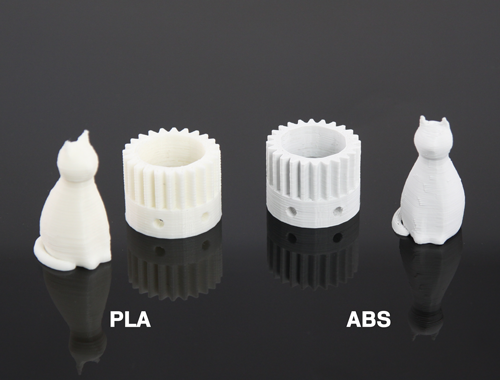
\includegraphics[width=0.41\textwidth,height=\textheight]{img/image_10.png}
\caption{Het zichtbare verschil tussen PLA en ABS\label{fig:plaabs}}
\end{figure}

\hypertarget{materialen-in-de-hand}{%
\subsection{Materialen in de hand}\label{materialen-in-de-hand}}

Er is ook ander materiaal nodig voor de prothesehand. Bijvoorbeeld
motortjes, draadjes, stroomdraadjes en een microcontroller of
microcomputer, deze sturen alles in de hand aan. Er zijn erg veel
verschillende motors op de markt. In een prothesehand heeft men deze het
liefst zo klein mogelijk, met toch aardig wat kracht. De ruimte is
namelijk minimaal en motors nemen al gauw flink wat ruimte in. Ook de
draad moet krachtig zijn. Visdraad is erg sterk en dun, wat het een
perfect materiaal maakt. De twee meest voorkomende microcontrollers
tegenwoordig zijn de Raspberry Pi en Arduino. Dit zijn de enige twee
controllers die zijn onderzocht, omdat het grootste marktaandeel uit
deze twee controllers bestaat. Raspberry Pi is een microcomputer en past
in je handpalm. Arduino heeft ook meerdere microcontrollers met deze
grootte, tevens hebben zij ook een nog kleinere microcontroller: de
Arduino Nano. Deze is de grootte van een pink. Dit maakt haar de
perfecte microcontroller voor een prothesehand. Het grote verschil is
dat de Nano geen poorten (USB, HDMI\ldots{}) heeft. Er kunnen dus niet
makkelijk USB-apparaten aan worden gekoppeld. Alles moet hierdoor via
pins, de metalen pinnetjes aan de onderkant in
\xrefname{Fig.}\cref{fig:nano}.

\begin{figure}
\centering
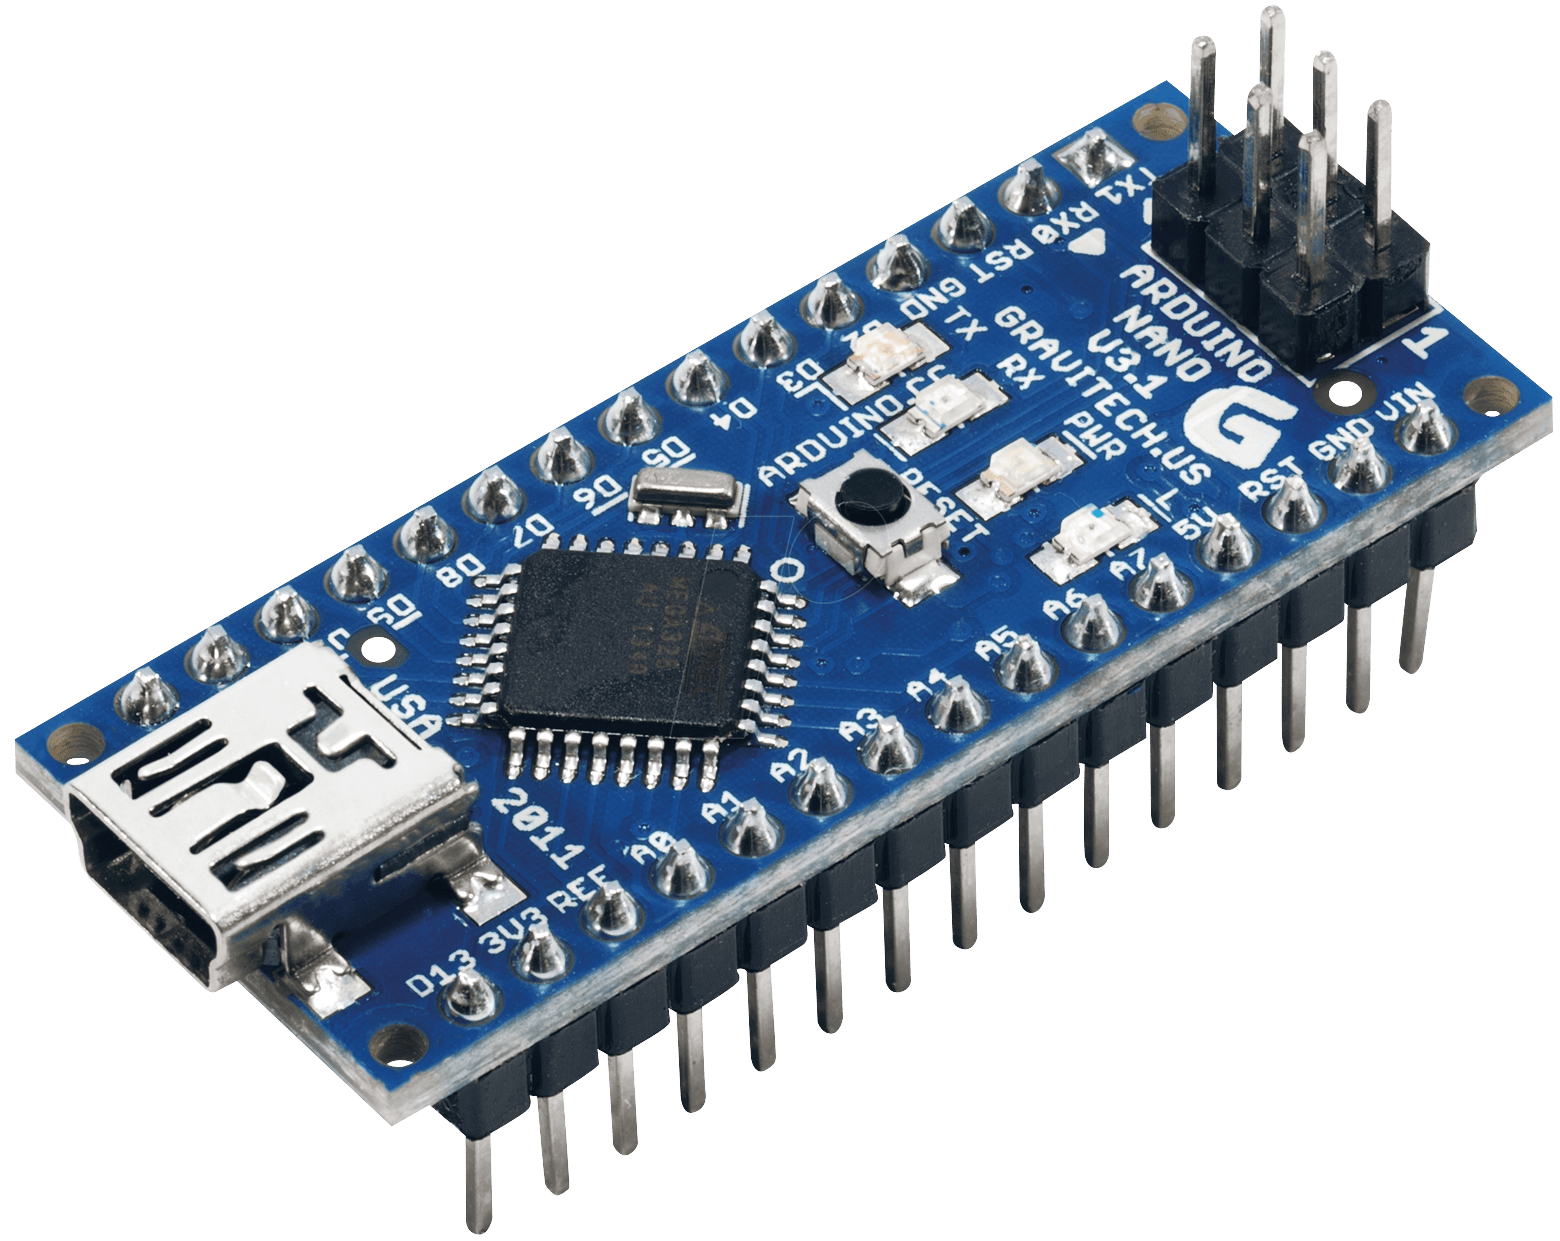
\includegraphics[width=0.36\textwidth,height=\textheight]{img/image_11.png}
\caption{De Arduino Nano v3\label{fig:nano}}
\end{figure}

\hypertarget{software}{%
\subsection{Software}\label{software}}

De software voor het productieproces wordt vooral bepaald door de
microcontroller. Vaak is een bepaalde microcontroller afhankelijk van
één programmeertaal en met een bepaald ontwikkelproces uitgedacht. Om
het simpel te houden gaat het nu verder in op de twee meest voorkomende
microcontrollers: de Raspberry Pi en de Arduino.

De Raspberry Pi is een microcontroller die draait op een speciale versie
van Linux (een open source\footnote{Software waarvan iedereen toegang
  heeft tot het bronmateriaal (de `source').} besturingssysteem),
genaamd Raspbian. Dit besturingssysteem of operating system (OS) is
speciaal ontwikkeld voor de Pi , zie Raspbian (z.d.). Gezien het feit
dat het een Unix-systeem is, werk je vooral met de terminal. Een
herkenbaar aspect van een dit systeem is de centrale rol van het
bestandssysteem (``Unix'' z.d.). Om met dit bestandssysteem te werken
maakt men gebruik van kleine programma's die gecombineerd worden in een
shell (\xrefname{Fig.}\cref{fig:shell}). Unix wordt vaak geassocieerd
met een `Command Line Interface'. Dit betekent dat de computer wordt
bestuurd met korte getypte opdrachten in plaats van het klikken op
knoppen en slepen van bestanden.

\begin{figure}
\centering
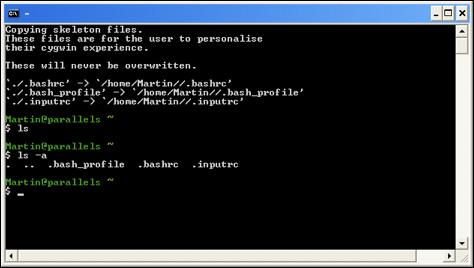
\includegraphics[width=0.55\textwidth,height=\textheight]{img/image_12.jpg}
\caption{Een voorbeeld van een Unix shell\label{fig:shell}}
\end{figure}

Verder ziet de Raspberry Pi er uit als een normale Windows computer, met
een bureaublad, applicaties, een browser en een dock. Over het algemeen
programmeer je Raspberry Pi's in Python. Dit is een in Nederland
ontwikkelde programmeertaal met een erg overzichtelijke syntax.

De Arduino is daarentegen geen microcomputer, maar een microcontroller ,
dit verschil wordt beschreven in Di Justo (2015). Dit verschil uit zich
in het niet hebben van een user interface (UI), te zien in
\xrefname{Fig.}\cref{fig:rpide}. Als men een Arduino dus via een
hdmi-kabel aan een extern beeldscherm hangt, gebeurt er niks. Een
Arduino is enkel bedoeld voor dingen als robotica en home automation
(het automatisch besturen van elektronische onderdelen van je huis). De
Arduino is daarentegen wel weer erg simpel in gebruik, vooral
gecombineerd met de Arduino IDE\footnote{Integrated Development
  Environment; de software die men gebruikt om software te ontwikkelen.}
(\xrefname{Fig.}\cref{fig:rpide}) (gebaseerd op Processing) en de
Arduino programmeertaal (gebaseerd op Wiring, Arduino Foundation
(2017)). Doordat de software, programmeertaal en hardware zo op elkaar
is afgestemd, gaat het proces een stuk makkelijker over het algemeen.

\begin{figure}
\centering
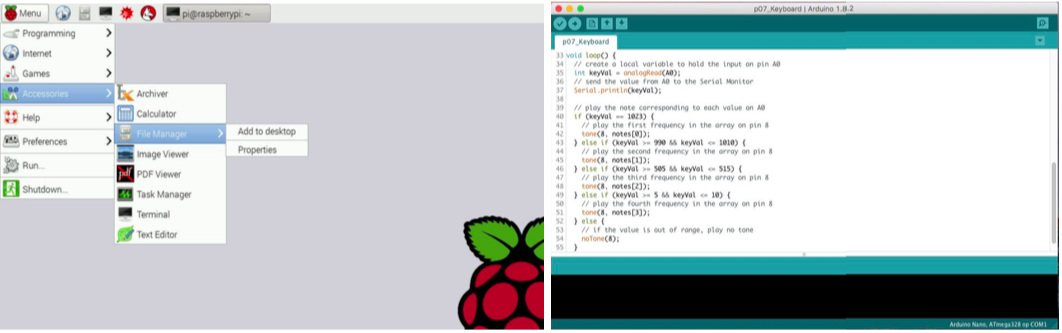
\includegraphics[width=1\textwidth,height=\textheight]{img/rpi_ard.png}
\caption{De Raspberry Pi UI naast de Arduino IDE\label{fig:rpide}}
\end{figure}

Voor programmeren is een goede, functionele IDE erg handig. Dit is
software om het ontwikkelen van software te vereenvoudigen. Een
veelgemaakte keuze hiervoor is de Atom text editor , te vinden in de
opsomming van Henry (2014). Dit is enkel een text editor, maar door de
vele packages die downloadbaar zijn, is Atom inmiddels volledig om te
bouwen tot uitgebreide IDE. Atom is ontwikkeld door Github, en daarom
ook volledig open source. Echter is Atom nog niet gebouwd voor
microcontrollers, zoals de Arduino IDE is. Hiervoor zijn packages
beschikbaar. PlatformIO, ontwikkeld door Kravets (2017), is hier een
van. Deze voegt verschillende tools en packages toe die het programmeren
van een microcontroller een stuk makkelijker maken. Zo kan men builden
(de code testen op fouten en omzetten naar C++) en uploaden (van de
computer naar de geheugenkaart van de microcontroller plaatsen),
rechtstreeks vanuit Atom. Atom met deze package is te zien in
\xrefname{Fig.}\cref{fig:atom}.

\begin{figure}
\centering
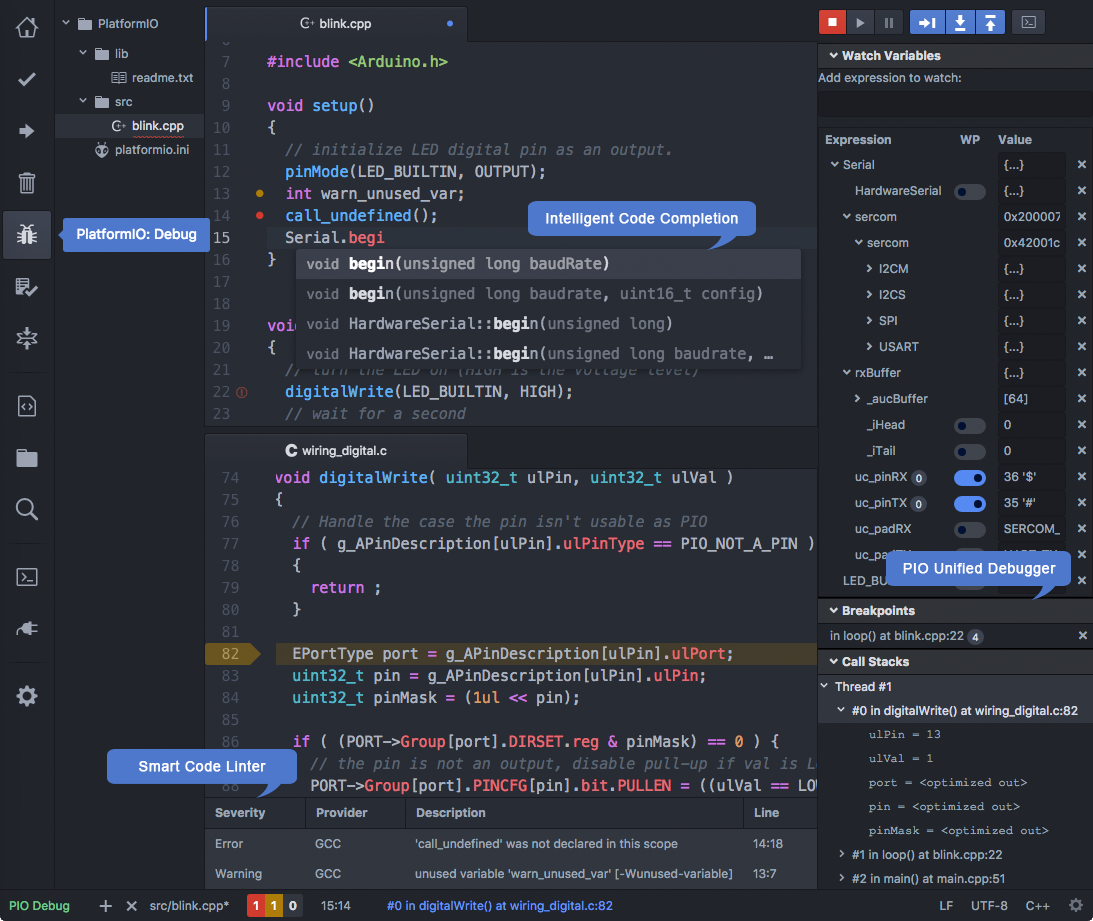
\includegraphics[width=0.5\textwidth,height=\textheight]{img/image_15.png}
\caption{Atom met PlatformIO package\label{fig:atom}}
\end{figure}

Het ontwerpen van 3D-afbeeldingen van de hand vereist ook speciale
software. Hiervoor zijn er erg veel verschillende applicaties, de meest
gebruikte zijn opgesomd in Duann (2012). Zo zijn er computerapplicaties,
maar ook webapplicaties. Deze applicaties hebben wat weg van Adobe
Photoshop. Het zijn over het algemeen programma's met veel tools, zoals
te zien is in \xrefname{Fig.}\cref{fig:123d}. Ook hebben deze
programma's vaak voorontworpen basisvormen, om het productieproces te
versnellen. Het kunnen zowel desktop applicaties als webapps zijn. Een
voorbeeld van een webapp hiervoor is Tinkercad. Het doel van Tinkercad
is het ontwerpen van 3d-afbeeldingen zo eenvoudig mogelijk te maken.
Tinkercad is dan ook geen complexe, professionele tool. Toch valt hier
bijna alles mee te maken.

\begin{figure}
\centering
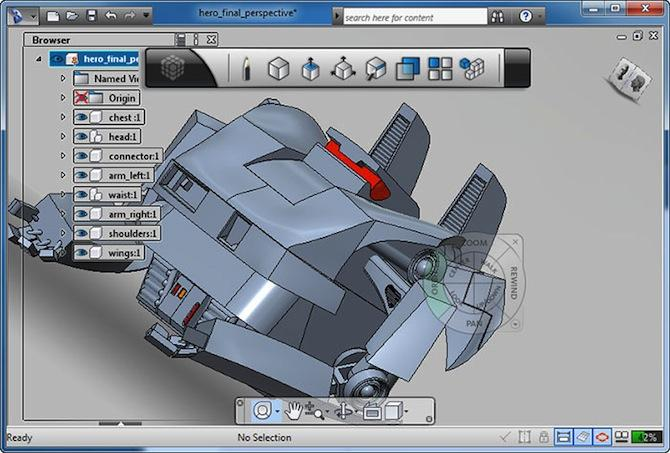
\includegraphics[width=0.6\textwidth,height=\textheight]{img/image_16.jpg}
\caption{Autodesk 123D software voor Windows\label{fig:123d}}
\end{figure}
